%% Ejemplo de la plantilla de latex para las diapositivas del Máster en IA 

%%%%%%%%%%%%%%%%%%%%%%%%%%%%
%% Valores para el ratio de aspecto: 43, 169 
\documentclass[10pt, envcountsect, presentation, aspectratio=169]{beamer}
%%%%%%%%%%%%%%%%%%%%%%%%%%%%

%%%%%%%%%%%%%%%%%%%%%%%%%%%%
%% Incluir fichero de estilo del máster
\input plantillaTAREA.sty
%%%%%%%%%%%%%%%%%%%%%%%%%%%%

\let\Tiny=\tiny
%\usepackage[latin1]{inputenc}
\usepackage[utf8]{inputenc}
\usepackage[spanish]{babel}
\usepackage{pgf}
\usepackage{latexsym}
\usepackage{amssymb,amsmath}
\usepackage{xspace}
\usepackage[olditem,oldenum]{paralist}
\usepackage{tikz}
\usetikzlibrary{snakes,arrows,shapes}
\usetikzlibrary{positioning}
\usetikzlibrary{arrows,automata}
\usepackage[T1]{fontenc}
\usepackage{psfrag}
\usepackage{multirow}
\usepackage{xmpmulti}
\usepackage[absolute, overlay]{textpos}
\usepackage{pgfpages}
\usepackage{pgf}
\usepackage{colortbl}
\usepackage{xcolor}
\usepackage{color}
\usepackage{booktabs}

%%%%%%%%%%%%%%%%%%%%%%%%%%%%
%% Información que aparecerá en la portada
\title[Nombre]{Modelos de Computación}
\subtitle{Entrega de Complejidad} % short title for footer

\author[Carrillo G., Gallego J., Ibarrola Y.] % Para el pie de página, poner los autores abreviados separados por comas.
{
	\sc{Ginés Carrillo Ibáñez}\\  % Autor 1
	\textit{Grupo 1. Subgrupo 9}\\
	\sc{Juan Diego Gallego Nicolás}\\ % Autor 2
	\textit{Grupo 1. Subgrupo 9}\\ 
	\sc{Yago Ibarrola Lapeña}\\ % Autor 3
	\textit{Grupo 1. Subgrupo 9}\\ 
}

\institute[GII]% % Poner las iniciales de los diferentes departamentos de los autores separadas por comas.
{
	\textit{Universidad de Murcia}
}

\date{2024/2025} % Curso académico

%%%%%%%%%%%%%%%%%%%%%%%%%%%%%%%%%%
%% Contenido de las diapositivas
\setbeamerfont{normal text}{size=\normalsize} % Modifica el tamaño del texto de las diapositivas.
\AtBeginDocument{\usebeamerfont{normal text}}

%%%%%%%%%%%%%%%%%%%%%%%%%%%%%%%%%%

\newcommand{\ldfa}{\ensuremath{\mathcal L_{DFA}}}
\newcommand{\lnfa}{\ensuremath{\mathcal L_{NFA}}}
\newcommand{\ler}{\ensuremath{\mathcal L_{ER}}}
\newcommand{\lreg}{\ensuremath{\mathcal {REG}}}
\newcommand{\lcf}{\ensuremath{\mathcal CF}}
\newcommand{\lpda}{\ensuremath{\mathcal L_{PDA}}}
\newcommand{\lpdav}{\ensuremath{\mathcal L_{PDA^v}}}
\newcommand{\lpdad}{\ensuremath{\mathcal L_{PDAD}}}
\newcommand{\lgr}{\ensuremath{\mathcal L_{GCF}}}
\newcommand{\ld}{\ensuremath{\mathcal {DEC}}}
\newcommand{\lr}{\ensuremath{\mathcal {RE}}}
\newcommand{\halt}{\ensuremath{\mathsf{HALT}}}
\newcommand{\fon}{\ensuremath{FO(\mathbb N)}}
\newcommand{\pol}{\ensuremath{\mathcal P}}
\newcommand{\npol}{\ensuremath{\mathcal{NP}}}
\newcommand{\cnpol}{\ensuremath{\mathcal{CO-NP}}}
\newcommand{\cnlo}{\ensuremath{\mathcal{CO-NLOG}}}
\newcommand{\cnpols}{\ensuremath{\mathcal{CO-NPSPACE}}}
\newcommand{\fo}{\ensuremath{FO}}
\newcommand{\lop}{\ensuremath{LP}}
\newcommand{\cnf}{\ensuremath{_{cnf}}}
\newcommand{\tcnf}{\ensuremath{_{3cnf}}}
%\newcommand{\cnf}{\ensuremath{LP_{cnf}}}
%\newcommand{\tcnf}{\ensuremath{LP_{3cnf}}}
\newcommand{\qlop}{\ensuremath{QLP}}
\newcommand{\dcnf}{\ensuremath{LP_{2cnf}}}
\newcommand{\pols}{\ensuremath{\mathcal{PSPACE}}}
\newcommand{\npols}{\ensuremath{\mathcal{NPSPACE}}}
\newcommand{\lo}{\ensuremath{\mathcal{LOG}}}
\newcommand{\nlo}{\ensuremath{\mathcal{NLOG}}}
\newcommand{\ext}{\ensuremath{\mathcal{EXPTIME}}}
\newcommand{\extn}{\ensuremath{\mathcal{NEXPTIME}}}
\newcommand{\exts}{\ensuremath{\mathcal{EXPSPACE}}}
\newcommand{\ej}{{\color{green}ejemplo}}
\newcommand{\usigma}{\ensuremath{\mathcal U}_{\Sigma}}
\newcommand{\mt}{\ensuremath{\mathcal {MT}}} 
\newcommand{\pnp}{¿\ensuremath{\mathcal{P}=\mathcal{NP}}? }
\newcommand{\ssum}{\ensuremath{SUBSET\text{-}SUM}}

%%%%%%%%%%%%%%%%%%%%%%%%%%%%%%%%%%

\begin{document}	

%%%%%%%%%%%%%%%%%%%%%%%%%%%%%%%%%%

%%%%%%%%%%%%%%%%%%%%%%%%%%%%%%%%%%

\begin{frame}[plain]
	\titlepage
\end{frame}

%%%%%%%%%%%%%%%%%%%%%%%%%%%%%%%%%%
\begin{frame}{Problema Decisional de la Suma de Subconjuntos}{Definición y lenguaje asociado}
    \textbf{Definición:} el problema de la suma de subconjuntos consiste en, dado un conjunto $X=\{x_1, \dots, x_k\}$ de enteros (posiblemente repetidos\footnote{El término para referirse a un conjunto que admite repetición es `multiconjunto'. Aun así, a lo largo de este documento nos referiremos a ellos como `conjuntos' por simplicidad.}) y un valor objetivo $t$, determinar si existe un subconjunto $S \subseteq X$ tal que $\sum _{x\in S}x = t$.\\~\\

    \textbf{Definición:} se define el lenguaje $\ssum$ como:
    $$
    \ssum:=\{\langle X, t \rangle \mid \exists \, S\subseteq X \text{ cumpliendo }\sum _{x\in S}x = t\}
    $$
    
    
\end{frame}
\begin{frame}{Problema Decisional de la Suma de Subconjuntos}{Ejemplos}
    \textbf{Ejemplos:}
    \begin{itemize}
        \item $\langle \{4, 4, 9\}, 8\rangle \in \ssum$, ya que  $4+4=8$.
        \item $\langle \{4, 4, 9\}, 11\rangle \notin \ssum$, ya que ningún subconjunto de $\{4, 4, 9\}$ suma 11
        \item $\langle X, 0\rangle \in \ssum$ trivialmente para un conjunto $X$ cualquiera\footnote{Consideramos $\sum_{x\in\emptyset} x = 0$.}.
        \item $\langle \{a, x_1, \dots, x_k\}, a\rangle \in \ssum$ trivialmente para cualquier $a$.
        \item $\langle \{2a_1,\dots,2a_k\}, t\rangle \notin \ssum$ para cualquier $t$ impar.
        \item $\langle \{2^0, \dots, 2^k\}, t\rangle \in \ssum$ para cualquier $0\leq t<2^{k+1}$.
        
    \end{itemize}
\end{frame}

\begin{frame}{Problema Decisional de la Suma de Subconjuntos}{El lenguaje $\ssum$ es $\mathcal{NP}-$completo}
    Para demostrar la $\mathcal{NP}-$completitud de $\ssum$ vamos a necesitar las siguientes propiedades que no demostramos:
    \begin{enumerate}[1]
        \item El lenguaje $3SAT$ formado por las formulas de lógica proposicional de la forma $\bigwedge_{i=1}^n(p_1^i \vee p_2^i \vee p_3^i)$ satisfacibles es $\mathcal{NP}-$completo.
        \item \textbf{Tercer Teorema de la Reducibilidad:} sean $L$ y $L'$ dos lenguajes con $L \leq_p L'$. Si $L$ es $\mathcal{NP}-$completo y $L'$ es $\mathcal{NP}$, entonces $L'$ es $\mathcal{NP}-$completo. 
    \end{enumerate}
    Si demostramos $\ssum \in \mathcal{NP}$ y $3SAT \leq_p \ssum$ tendremos el resultado que buscamos. 
\end{frame}

\begin{frame}{Problema Decisional de la Suma de Subconjuntos}{El lenguaje $\ssum$ es $\mathcal{NP}$}

    \textbf{Proposición:} $\ssum \in \mathcal{NP}$\\~\\
    \textbf{Demostración:} construiremos una máquina de Turing $V_{\ssum}$ que verifique una solución de $\ssum$ en tiempo polinomial.\\
    Dada una entrada $\langle \langle X, t\rangle, S\rangle$, $V_{\ssum}$ actúa como sigue:
    \begin{enumerate}
        \item Comprueba que $S$ es un conjunto de enteros con suma $t$. Si no, RECHAZA.
        \item Comprueba que $S$ es un subconjunto de $X$. Si no, RECHAZA.
        \item ACEPTA
    \end{enumerate}
    Puesto que $V_{\ssum}$ termina su ejecución en tiempo polinomial, tenemos $\ssum \in \mathcal{NP}$\, como queríamos ver.
\end{frame}

\begin{frame}{Problema Decisional de la Suma de Subconjuntos}{El lenguaje $3SAT$ se polirreduce a $\ssum$}

    \textbf{Proposición:} $3SAT \leq_p \ssum$ \\~\\
    \textbf{Demostración:} si especificamos un algoritmo para, dada una fórmula $3cnf$ arbitraria $\Phi$, construir (en tiempo polinomial) un problema de suma de subconjuntos $\langle X, t\rangle$ tal que $\langle X, t\rangle \in \ssum \iff  \Phi \in 3SAT$, la proposición quedaría demostrada.\\~\\
    La demostración continúa en las siguientes diapositivas.
    
\end{frame}
\begin{frame}{Problema Decisional de la Suma de Subconjuntos}{El lenguaje $3SAT$ se polirreduce a $\ssum$}
    Sea $\Phi = \bigwedge_{i=1}^k(p_{a_i} \vee p_{b_i} \vee p_{c_i})$ una fórmula de $l$ variables, donde $a_i,b_i, c_i\in\{1,\dots, l\}\, \forall i \in 1,\dots,k$. Llamemos también $d_i$ a la i-ésima disyunción de la fórmula, es decir, $d_i = (p_{a_i} \vee p_{b_i} \vee p_{c_i})$\\~\\
    Para cada variable $p_i$ añadimos a $X$ dos enteros, que denotaremos $y_i$ y $z_i$. Para cada disyunción $d_i$ añadimos otros dos enteros, $g_i$ y $h_i$.\\
    \begin{itemize}
        \item $y_i$ tendrá $k + l - i + 1$ cifras. Su dígito más significativo será un $1$, seguido de $l-i$ ceros. Numeremos ahora las $k$ cifras restantes de izquierda a derecha (de $1$ a $k$). La cifra $j$ de $y_i$ será un $1$ si $d_j$ hace referencia a la variable $p_i$ (sin negar). Si no, será $0$.
        \item $z_i$ se construye de manera igual a $y_i$, salvo que sus últimas $k$ cifras son $1$ si la disyunción correspondiente hace referencia a $\neg p_i$, en lugar de $p_i$.
        \item $g_i$ y $h_i$ serán ambas un $1$ seguido de $k-i$ ceros.
        \item $t$ estará compuesto de $l$ unos seguido de $k$ treses.
    \end{itemize}
\end{frame}

\begin{frame}{Problema Decisional de la Suma de Subconjuntos}{Ejemplo}
    \begin{columns}
        \column{0.5\textwidth}
        La mejor forma de entender la construcción es mediante un ejemplo:\\~\\
        Sea $\Phi = (p_{1} \vee p_{2} \vee p_{3})\wedge (\neg p_{1} \vee p_{2} \vee \neg p_{3})$\\~\\
        Aquí, $k=2$ y $l=3$, luego las variables $x_i$, $y_i$, $g_i$, $h_i$ y $t$ toman los valores que se muestran en la tabla.\\~\\
        \textbf{Observación:} Nótese que por la construcción de $X$, ningún subconjunto suyo producirá una suma con llevadas (en cada posición habrá, como mucho, $5$ unos).
        \column{0.5\textwidth}
        \small
        \begin{center}
        \renewcommand{\arraystretch}{1.2}
        \begin{tabular}{l|*{3}{c}|*{2}{c}}
         & $p_1$ & $p_2$ & $p_3$ & $d_1$ & $d_2$ \\
        \midrule
        $y_1$ & 1 & 0 & 0 & 1 & 0 \\
        $z_1$ & 1 & 0 & 0 & 0 & 1 \\
        $y_2$ &   & 1 & 0 & 1 & 1 \\
        $z_2$ &   & 1 & 0 & 0 & 0 \\
        $y_3$ &   &   & 1 & 1 & 0 \\
        $z_3$ &   &   & 1 & 0 & 1 \\
        \midrule
        $g_1$ &   &   &   & 1 & 0 \\
        $h_1$ &   &   &   & 1 & 0 \\
        $g_2$ &   &   &   &   & 1 \\
        $h_2$ &   &   &   &   & 1 \\
        \midrule
        $t$   & 1 & 1 & 1 & 3 & 3 \\
        \end{tabular}
        \end{center}
    \end{columns}
\end{frame}



\begin{frame}{Problema Decisional de la Suma de Subconjuntos}{El lenguaje $3SAT$ se polirreduce a $\ssum$}
    Veamos ahora que $\langle X, t\rangle \in \ssum \iff  \Phi \in 3SAT$:\\~\\
    \boxed{\Rightarrow} Sea $S$ el subconjunto de $X$ de suma $t$. Es fácil ver que para cualquier $i\in\{1,\dots,l\}$, exactamente uno de entre $y_i$ y $z_i$ pertenecerá a $S$ (recordemos que no hay llevadas). Asignemos a $p_i$ el valor $TRUE$ si $y_i=1$ y $FALSE$ si $z_i=1$. \\~\\
    Necesariamente, la asignación realizada satisface $\Phi$, por el siguiente razonamiento:\\
    Para cada disyunción, su dígito asociado en la suma debe ser igual a $3$. Dado que de los $g_i$ y $h_i$ solo se pueden obtener $2$ unos, el tercero debe venir de uno de los $y_i$ o $z_i$ de $S$. Pero entonces, por construcción, el valor de verdad de $p_i$ hará que esa disyunción se evalúe a $TRUE$.\\~\\
    \boxed{\Leftarrow} Tenemos una asignación de variables que satisface $\Phi$. Construimos $S$ de la siguiente forma:\\
    Si $p_i = TRUE$, $y_i\in S$, si no, $z_i\in S$. De esta forma, las $l$ primeras cifras de la suma son $1$. Puesto que la asignación satisface $\Phi$, tendremos una suma de al menos $1$ en cada uno de los últimos $k$ dígitos. Finalmente tomamos los $g_i$ y $h_i$ que sean necesarios hasta que la suma total sea igual a $t$.
    
\end{frame}

\begin{frame}{Problema Decisional de la Suma de Subconjuntos}{El lenguaje $\ssum$ es $\mathcal{NP}-$completo}
    Finalmente, es sencillo comprobar que esta construcción se puede realizar en tiempo polinomial (particularmente, del orden de $(k+l)^2$ operaciones sencillas).\\~\\
    Hemos obtenido, por tanto, una polirreducción de $3SAT$ a $\ssum$, como buscábamos. \\~\\ 

    Aplicando directamente el \textbf{Tercer Teorema de la Reducibilidad}, tenemos que $\ssum \in \mathcal{NP}-$completo. $\boxed{ }$
\end{frame}


%%%%%%%%%%%%%%%%%%%%%%%%%%%%%%%%%%

\begin{frame}{Problema Decisional de la Clique en un Grafo No Dirigido}{$k-clique$}
    % \vskip -1cm % Para subir (-) o bajar el texto
    \textbf{Definición:} dado un grafo no dirigido $G=(V,E)$ y un entero positivo $k$, un $k-clique$ es un subgrafo de $G$ que es completo. $G'=(V',E') \subseteq (V,E)$ es $k-clique$ de $G \Leftrightarrow |E'| = \frac{|V'|(|V'|-1)}{2} \Leftrightarrow$ $\forall v, w \in V', v \neq w \text{ } (v,w)\in E'$. Un $k-clique$ también puede recibir el nombre de $clique$ de orden $k$. \\~\\

    \textbf{Propiedades:}

    \begin{itemize}
        \item[] Todo grafo no vacío tiene al menos un $1-clique$
        \item[] Todo grafo $G=(V,E)$ con $E \neq \emptyset$ tiene al menos un $2-clique$
        \item[] Si un grafo tiene un $k-clique$, tiene $cliques$ de todos los órdenes de $1$ 
        \item[] Todo grafo completo de $n$ vértices tiene $cliques$ de todos los órdenes de $1$ a $n$
    \end{itemize}
    
\end{frame}

\begin{frame}{Problema Decisional de la Clique en un Grafo No Dirigido}{$k-clique$}
    % \vskip -1cm % Para subir (-) o bajar el texto
    En el siguiente grafo podemos encontrar cliques de órdenes de $1$ hasta $4$:
    \begin{figure}
        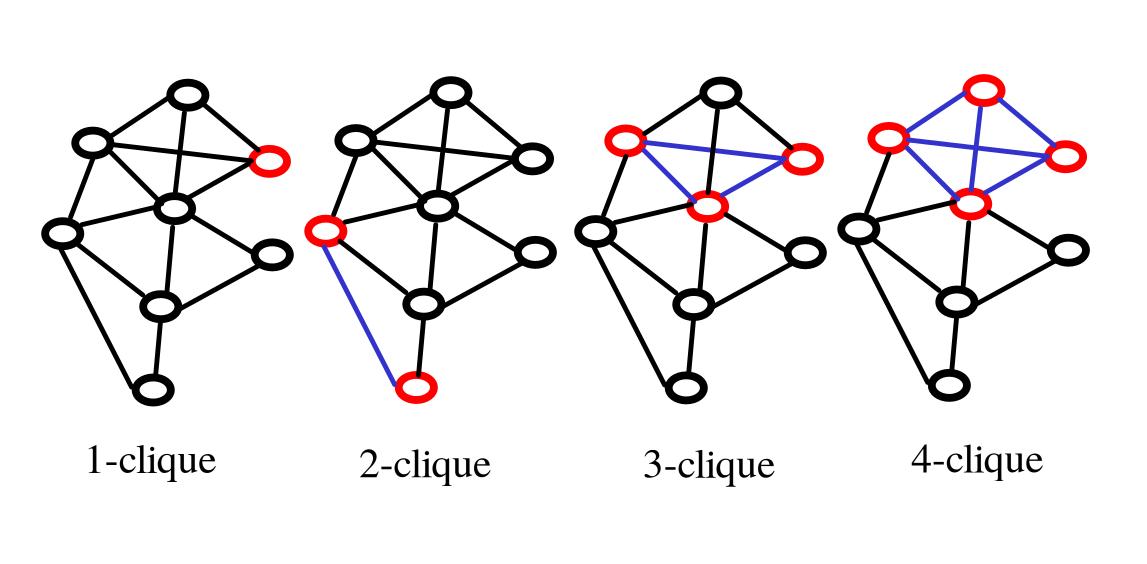
\includegraphics[scale=0.25]{images/T2_2_ejemploclique.png}
    \end{figure} 
\end{frame}

\begin{frame}{Problema Decisional de la Clique en un Grafo No Dirigido}{El lenguaje $K-CLIQUE$}
    % \vskip -1cm % Para subir (-) o bajar el texto
    \textbf{Definición:} se define el lenguaje $K-CLIQUE$ como:
    $$
    K-CLIQUE:=\{\langle G \rangle \mid G \text{ es un g.n.d. con un } K-clique\}
    $$

    \textbf{Proposición:} $K-CLIQUE \in \mathcal{P} \text{  } \forall K>0$ \\
    \textbf{Demostración:} basta diseñar una $MT$ que compruebe las $\binom{|V|}{k} = \frac{|V|!}{k!(|V|-k)!}=O(|V|^k)$ posibles combinaciones sin repetición de nodos del grafo codificado. Sea $M_K$ la $MT$ que ante una entrada $\langle G \rangle$:
    \begin{enumerate}[I]
        \item Decodifica la entrada
        \item Si $|V|<K$ RECHAZA
        \item Para cada subconjunto $V_K\subseteq V$ de $K$ vértices de $G=(V,E)$ comprobar si existe una arista en $E$ para cada par de vértices distintos de $V_K$.
        \item Si algún $V_K$ no cumple la condición RECHAZA, sino ACEPTA
    \end{enumerate}
    Como $|E|<|V|^2$, se trata de una máquina determinista con complejidad polinómica.
\end{frame}

\begin{frame}{Problema Decisional de la Clique en un Grafo No Dirigido}{El lenguaje $CLIQUE$}
    % \vskip -1cm % Para subir (-) o bajar el texto
    \textbf{Definición:} se define el lenguaje $CLIQUE$ como:
    $$
    CLIQUE:=\{\langle G, k \rangle \mid G \text{ es un g.n.d. con un } k-clique\}
    $$
    Por la diapositiva anterior, pudiera parecer que $CLIQUE \in \mathcal{P}$ trivialmente.
    No obstante, veremos más adelante que el lenguaje es $\mathcal{NP}-$completo. Primero veamos que es $\mathcal{NP}$ \\~\\

    \textbf{Proposición:} $CLIQUE \in \mathcal{NP}$

    \textbf{Demostración: } Sea $M_{CLIQUE}$ la $MT$ no determinista que ante una entrada $\langle G, k \rangle$:

    \begin{enumerate}[I]
        \item Elige un subconjunto $V_k \subseteq V$ de $k$ vértices de $G=(V,E)$
        \item Comprueba que hay un arco entre cada par de vértices de $V_k$
    \end{enumerate}

    Por el mismo razonamiento que en el caso de $M_K$, $M_{CLIQUE}$ es una $MTND$.
\end{frame}

\begin{frame}{Problema Decisional de la Clique en un Grafo No Dirigido}{El lenguaje $CLIQUE$ es $\mathcal{NP}-$completo}
    Para demostrar la $\mathcal{NP}-$completitud de $CLIQUE$ vamos a necesitar las siguientes propiedades que no demostramos:
    \begin{enumerate}[1]
        \item El lenguaje $3SAT$ formado por las formulas de lógica proposicional de la forma $\bigwedge_{i=1}^n(p_1^i \vee p_2^i \vee p_3^i)$ satisfacibles es $\mathcal{NP}-$completo.
        \item \textbf{Tercer Teorema de la Reducibilidad:} sean $L$ y $L'$ dos lenguajes con $L \leq_p L'$. Si $L$ es $\mathcal{NP}-$completo y $L'$ es $\mathcal{NP}$, entonces $L'$ es $\mathcal{NP}-$completo. 
    \end{enumerate}
    Si demostramos $3SAT \leq_p CLIQUE$ tendremos el resultado que buscamos. 
\end{frame}

\begin{frame}{Problema Decisional de la Clique en un Grafo No Dirigido}{El lenguaje $CLIQUE$ es $\mathcal{NP}-$completo}
    Sea $\Phi=\bigwedge_{i=1}^n(p_1^i \vee p_2^i \vee p_3^i)$ una fórmula proposicional cualquiera. Sea $M$ la $MT$ que toma como entrada $\Phi$ y construye un grafo $G_\Phi$:
    \begin{enumerate}
        \item Para cada $i=1,\dots,n$, crea un grupo de tres vértices $V_{p_1^i}, V_{p_2^i}, V_{p_3^i}$
        \item Crea una arista entre cualquier par de véctices $V_{p_a^i}$, $V_{p_b^j}$ que cumpla:
        \begin{itemize}
            \item[] $i \neq j$
            \item[] $p_a^i \neq \neg p_b^j$ (como variables)
        \end{itemize}
    \end{enumerate}
    Es decir, crea 3 nodos por cláusula (uno por literal) y conecta cada nodo con todos los nodos de otras cláusulas con los que no haya un conflicto lógico.
    Es claro que el proceso de generación del grafo es polinomial con respecto al número de cláusulas de $\Phi$
\end{frame}

\begin{frame}{Problema Decisional de la Clique en un Grafo No Dirigido}{El lenguaje $CLIQUE$ es $\mathcal{NP}-$completo}
    Tomemos como ejemplo la fórmula de la tarea: 
    $$
    \Phi = (p_1 \vee p_2 \vee p_3) \wedge (\neg p_2 \vee p_3 \vee p_4) \wedge (p_3 \vee p_4 \vee p_5) \wedge(\neg p_4 \vee \neg p_5 \vee p_6)
    $$
    Aplicando el proceso definido en la diapositiva anterior, el grafo $G_\Phi$ es el complementario al siguiente\footnote{Es más fácil de visualizar el complementario ya que el grafo tiene muchos vértices}:
    \begin{figure}
        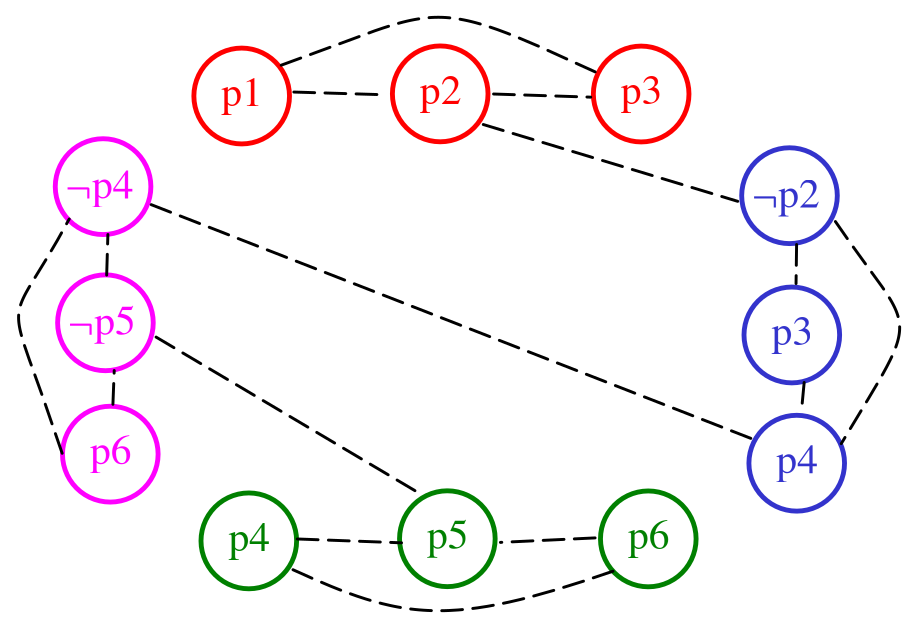
\includegraphics[scale=0.15]{images/T2_2_ejemplophi.png}
    \end{figure} 
\end{frame}

\begin{frame}{Problema Decisional de la Clique en un Grafo No Dirigido}{El lenguaje $CLIQUE$ es $\mathcal{NP}-$completo}
    \textbf{Teorema:} Dado un entero $k>0$ y $\Phi=\bigwedge_{i=1}^k(p_1^i \vee p_2^i \vee p_3^i)$ una proposición, $\Phi \in 3SAT \Leftrightarrow G_\Phi$ tiene un $k-clique$ \\~\\

    \textbf{Demostración:} \\
    $\boxed{\Rightarrow}$ Si $\Phi$ es satisfacible. Elegimos un literal $p_i^{a_i}$ para cada $i=1,\dots,k$ ($a_i=1,2,3$). Los vértices $V_{p_1^{a_1}},\dots,V_{p_k^{a_k}}$ deben tener todos aristas entre si pues todas los literales pertenecen a cláusulas distintas y no pueden ser contradictorios.
    Por tanto, el grafo completo formado por dichos vértices es un $k-clique$ de $G_\Phi \in CLIQUE$.

    $\boxed{\Leftarrow}$ De igual manera, si $G_\Phi$ es un grafo con un $k-clique$, este debe estar formado por vértices que corresponden a literales de cláusulas distintas y no contradictorios dos a dos.
    Estos literales tomados como verdaderos forman una asignación satisfactoria para $\Phi$ con lo que $Phi \in 3SAT$.
\end{frame}

\begin{frame}{Problema Decisional de la Clique en un Grafo No Dirigido}{El lenguaje $CLIQUE$ es $\mathcal{NP}-$completo}
    En suma, la aplicación que transforma una proposición $\Phi=\bigwedge_{i=1}^k(p_1^i \vee p_2^i \vee p_3^i)$ en una grafo $G_\Phi$ es polinómica y cumple $Phi \in 3SAT \Leftrightarrow G_\Phi \in CLIQUE$. Esto significa que es una polirreducción. \\~\\ 

    Aplicando directamente el \textbf{Tercer Teorema de la Reducibilidad}, $G_\Phi \in \mathcal{NP}-$completo. $\boxed{ }$
\end{frame}


%%%%%%%%%%%%%%%%%%%%%%%%%%%%%%%%%%

\begin{frame}{Problema Decisional de la Cobertura de Vértices}{Cobertura de vértices}
    % \vskip -1cm % Para subir (-) o bajar el texto
    \textbf{Definición:} dado un grafo no dirigido $G=(V,E)$ una cobertura de vértices de G es un subconjunto  $V' \subset V$ tal que $\forall v, w \in V, v \neq w \text{ } (v,w)\in E$ se cumple que $v \in V'$ o bien $w\in V'$, es decir, todas las aristas de G tienen al menos un extremo tocando un vértice de $V'$.
     \\~\\

    \textbf{Ejemplo:}

    \begin{itemize}
        \item[] El conjunto de todos los vértices es una cobertura de vértices.
    \end{itemize}

    \textbf{Propiedad:}

    \begin{itemize}
        \item[] Un conjunto de vértices es una cobertura de vértices si y solo si su complemento es un conjunto independiente, es decir, ninguno de sus vértices es adyacente.
    \end{itemize}
    
\end{frame}


%%%%%%%%%%%%%%%%%%%%%%%%%%%%%%%%%%

\begin{frame}{Problema Decisional de la Cobertura de Vértices}{Cobertura de vértices}
    % \vskip -1cm % Para subir (-) o bajar el texto
    En el siguiente grafo podemos encontrar varios coberturas de vértices, con distinto número de nodos seleccionados:
    \begin{figure}
        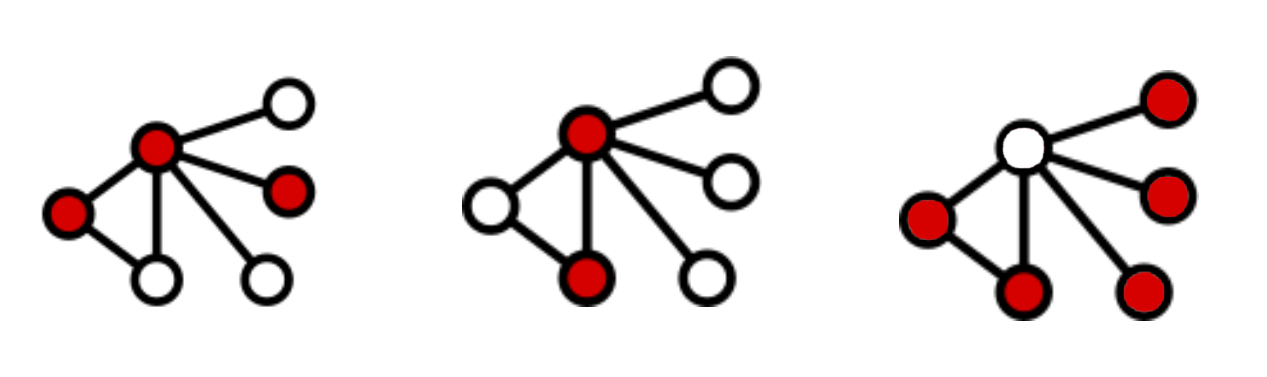
\includegraphics[scale=0.25]{images/T2_3_ejemploCoberturaVertices.png}
    \end{figure} 
\end{frame}

\begin{frame}{Problema Decisional de la Cobertura de Vértices}{Cobertura de vértices}
    % \vskip -1cm % Para subir (-) o bajar el texto
    Sin embargo, estos subconjuntos de vértices no forman una cobertura de vértices, pues las aristas señaladas con la flecha no tienen ningún de sus extremos en el subconjunto:
    \begin{figure}
        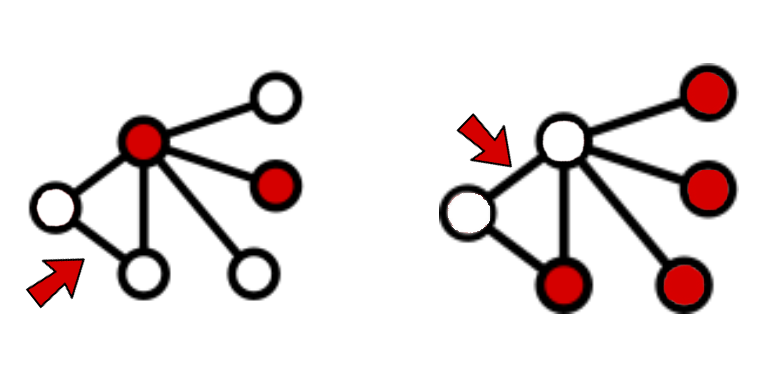
\includegraphics[scale=0.25]{images/T2_3_ejemploFalloCobertura.png}
    \end{figure} 
\end{frame}

\begin{frame}{Problema Decisional de la Cobertura de Vértices}{El lenguaje $VERTEX-COVER$}
    % \vskip -1cm % Para subir (-) o bajar el texto
    \textbf{Definición:} se define el lenguaje $VERTEX-COVER$ como:
    $$
    VERTEX-COVER:=\{\langle G, k \rangle \mid G \text{ es un g.n.d. con una cobertura de vértices formada por k nodos}\}
    $$
    

    \textbf{Proposición:} $VERTEX-COVER \in \mathcal{NP}$

    \textbf{Demostración: } Sea $M_{VERTEX-COVER}$ la $MT$ no determinista que ante una entrada $\langle G, k \rangle$:

    \begin{enumerate}[I]
        \item Elige un subconjunto $V_k \subseteq V$ de $k$ vértices de $G=(V,E)$
        \item Comprueba que toda arista de E tiene un extremo en $V_k$
        \item Si es así ACEPTA, y si no, RECHAZA
    \end{enumerate}

    Una vez tenemos la cobertura de vértices de tamaño k, la comprobación es polinomial, pues se deben verificar $|E|$ aristas para asegurar que al menos uno de los extremos pertenece al subconjunto elegido.
    Es por tanto una MTND con complejidad polinómica.

\end{frame}

\begin{frame}{Problema Decisional de la Cobertura de Vértices}{El lenguaje $VERTEX-COVER$ es $\mathcal{NP}-$completo }
    % \vskip -1cm % Para subir (-) o bajar el texto
    \textbf{Teorema:} El lenguaje $VERTEX-COVER$ es $ \mathcal{NP}-$completo
    

    \textbf{Demostración: } 
    
    Ya hemos visto que $VERTEX-COVER \in \mathcal{NP}$. Vamos a ver ahora la completitud. 
    
    Para ello vamos a utilizar las siguientes propiedades, que no se demostrarán:
    \begin{enumerate}[1]
        \item El lenguaje $3SAT$ formado por las formulas de lógica proposicional de la forma $\bigwedge_{i=1}^n(p_1^i \vee p_2^i \vee p_3^i)$ satisfacibles es $\mathcal{NP}-$completo.
        \item \textbf{Tercer Teorema de la Reducibilidad:} sean $L$ y $L'$ dos lenguajes con $L \leq_p L'$. Si $L$ es $\mathcal{NP}-$completo y $L'$ es $\mathcal{NP}$, entonces $L'$ es $\mathcal{NP}-$completo. 
    \end{enumerate}
    Si demostramos $3SAT \leq_p VERTEX-COVER$ tendremos el resultado que buscamos. 
    

\end{frame}


\begin{frame}{Problema Decisional de la Cobertura de Vértices}{El lenguaje $VERTEX-COVER$ es $\mathcal{NP}-$completo }
    Sea $\Phi=\bigwedge_{i=1}^n(p_1^i \vee p_2^i \vee p_3^i)$ una fórmula proposicional cualquiera. Sea $M$ la $MT$ que toma como entrada $\Phi$ y construye un grafo $G_\Phi$:
    \begin{enumerate}
        \item Para cada proposicion $p$ que aparece en $\Phi$, producimos un subgrafo formado por una arista uniendo dos vértices, a los que nombramos $p$ y $\overline{p}$. Cada uno de estos subgrafos, que se añaden a $G_\phi$, recibe el nombre de \textbf{subgrafo-variable }$p$.

        \item Para cada cláusula en $\Phi$, se producirá un grafo formado por una tripla de nodos conectados entre sí. Este subgrafo, llamado \textbf{subgrafo-cláusula} se añade también a $G_\phi$.

        \item Los tres nodos de cada subgrafo-cláusula se conectan también a los nodos de los subgrafos-variable que tienen su mismo identificador.
    \end{enumerate}
    Por tanto, el número total de nodos del grafo $G_\phi$ es $2m + 3l$, siendo m el número de proposiciones y l el número de cláusulas de $\Phi$. Se tomará $k = m + 2l$

    Evidentemente, el proceso de generación del grafo es polinomial con respecto al número de cláusulas de $\Phi$.
\end{frame}

\begin{frame}{Problema Decisional de la Cobertura de Vértices}{El lenguaje $VERTEX\text{-}COVER$ es $\mathcal{NP}-$completo}
    \centering
    Vemos las tres formas de construcción del grafo $G_\phi$:
    
    \begin{minipage}{0.32\textwidth}
        \centering
        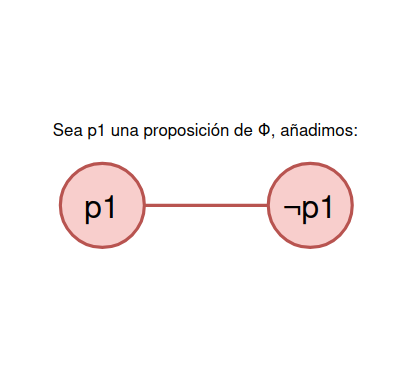
\includegraphics[width=\linewidth]{images/image.png}
        \\\small Subgrafo de variable
        
    \end{minipage}
    \hfill
    \begin{minipage}{0.32\textwidth}
        \centering
        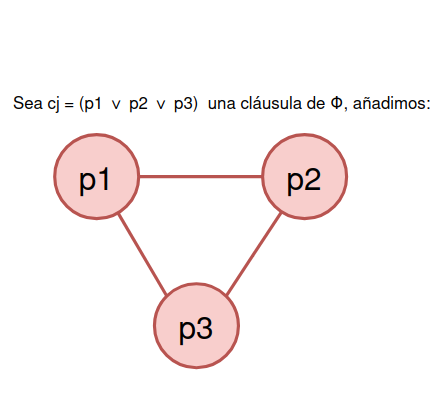
\includegraphics[width=\linewidth]{images/image2.png}
        \\\small Subgrafo de cláusula
    \end{minipage}
    \hfill
    \begin{minipage}{0.32\textwidth}
        \centering
        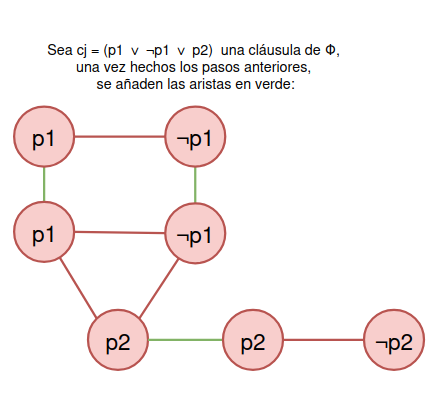
\includegraphics[width=\linewidth]{images/image3.png}
        \\\small Últimas aristas
    \end{minipage}
\end{frame}


\begin{frame}{Problema Decisional de la Cobertura de Vértices}{El lenguaje $VERTEX\text{-}COVER$ es $\mathcal{NP}-$completo}
    \centering
    Veamos un ejemplo completo.

    Sea $\Phi = (p1 \vee p2 \vee p2) \wedge  (\overline{p1} \vee \overline{p1} \vee p2)\wedge  (\overline{p2} \vee p1 \vee p1)$

    El grafo $G_\Phi$ resultante sería:
    \begin{figure}
        \centering
        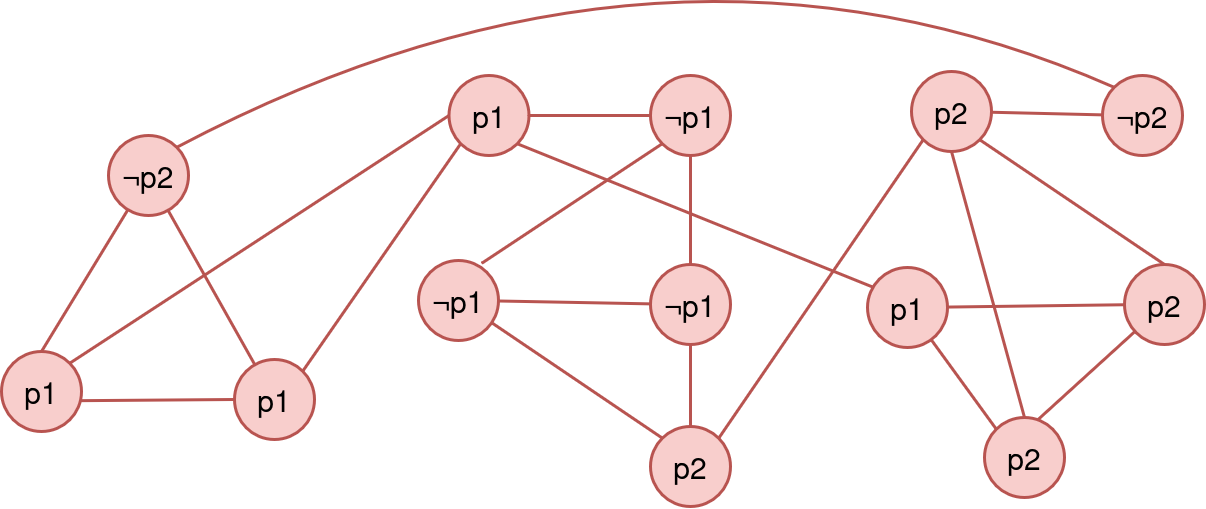
\includegraphics[width=0.65\linewidth]{images/T2_3_ejemploGrafo.png}
        \caption{Grafo $G_\Phi$}
        \label{fig:enter-label}
    \end{figure}
\end{frame}


\begin{frame}{Problema Decisional de la Cobertura de Vértices}{El lenguaje $VERTEX\text{-}COVER$ es $\mathcal{NP}-$completo}
    \textbf{Teorema:} Sea $\Phi=\bigwedge_{i=1}^k(p_1^i \vee p_2^i \vee p_3^i)$ una proposición, $\Phi \in 3SAT \Leftrightarrow G_\Phi$  tiene una cobertura de vértices con k vértices. \\~\\

    \textbf{Demostración:} \\
    $\boxed{\Rightarrow}$ Si $\Phi$ es satisfacible. Añadimos a la cobertura de vértices los nodos de los subgrafos-variable cuyo literal está a True. 
    Ahora, en cada subgrafo-cláusula seleccionamos un nodo cuyo literal esté a True y añadimos los dos nodos restantes a la cobertura. Así, ya tenemos $k = 2m + l$ nodos en la cobertura (m es el número de cláusulas y l el número de proposiciones de $\Phi$).
    Claramente, las aristas de los subgrafos-variable están cubiertas, al igual que las de los subgrafos-cláusula. Ahora, también se cubren las aristas entre los dos tipos de subgrafos, pues:
    \begin{itemize}
        \item Si $p_i$ es True, todas las aristas de la forma $(p_i,p_i)$ están cubiertas por el vértice del subgrafo-variable (Análogo para $\overline{p_i} = True$)
        \item Si $p_i$ es False, entonces en los subgrafos cláusula donde aparezca no la habremos descartado y las aristas $(p_i,p_i)$ estarán cubiertas por el nodo del correspondiente subgrafo-cláusula.
    \end{itemize}
    Por tanto, el grafo $G_\Phi \in VERTEX-COVER$
    
\end{frame}


\begin{frame}{Problema Decisional de la Cobertura de Vértices}{El lenguaje $VERTEX\text{-}COVER$ es $\mathcal{NP}-$completo}
    \textbf{Teorema:} Sea $\Phi=\bigwedge_{i=1}^k(p_1^i \vee p_2^i \vee p_3^i)$ una proposición, $\Phi \in 3SAT \Leftrightarrow G_\Phi$  tiene una cobertura de vértices con k vértices. \\~\\

    \textbf{Demostración:} \\
    $\boxed{\Leftarrow}$ De igual manera, si $G_\Phi$ es un grafo con con una cobertura de $k=2m+l$ nodos, podemos mostrar que $\Phi$ es satisfacible construyendo la asignación que lo satisface.
    La cobertura del grafo $G_\Phi$ debe contener un nodo en cada subgrafo-variable y dos en cada subgrafo-cláusula para cubrir todas las aristas de los dos tipos de subgrafo. De esta manera ya tenemos los k nodos que formarían parte de la cobertura. 

    Ahora tomamos los nodos de los subgrafos-variable que están el la cobertura y asignamos True a su literal. Esta asignación satisface $\Phi$ ya que hay tres aristas conectando los nodos de cada subgrafo-cláusula con los nodos de los subgragos-variable. Pero sabemos que en cada subgrafo-cláusula solo dos nodos están en $G_ \Phi$. Por tanto, la tercera arista debe cubrirse con un nodo del subgrafo-variable que esté en $G_\Phi$. Entonces, como a estos nodos le habíamos asignado True a su literal, tenemos que se cumple la cláusula correspondiente. Esto se puede aplicar a todas las cláusulas de $\Phi$, por lo que concluimos que $\Phi$ es satisfacible.
\end{frame}

\begin{frame}{Problema Decisional de la Cobertura de Vértices}{El lenguaje $VERTEX\text{-}COVER$ es $\mathcal{NP}-$completo}
    \centering
    Con el ejemplo anterior, podemos ilustrar la creación de la cobertura de k nodos.

    Sea $\Phi = (p1 \vee p2 \vee p2) \wedge  (\overline{p1} \vee \overline{p1} \vee p2)\wedge  (\overline{p2} \vee p1 \vee p1)$
    
    Esta proposición es satisfacible con $p1 = True$ y $p2 = True$
    
    La cobertura serían los vértices marcados en verde:
    \begin{figure}
        \centering
        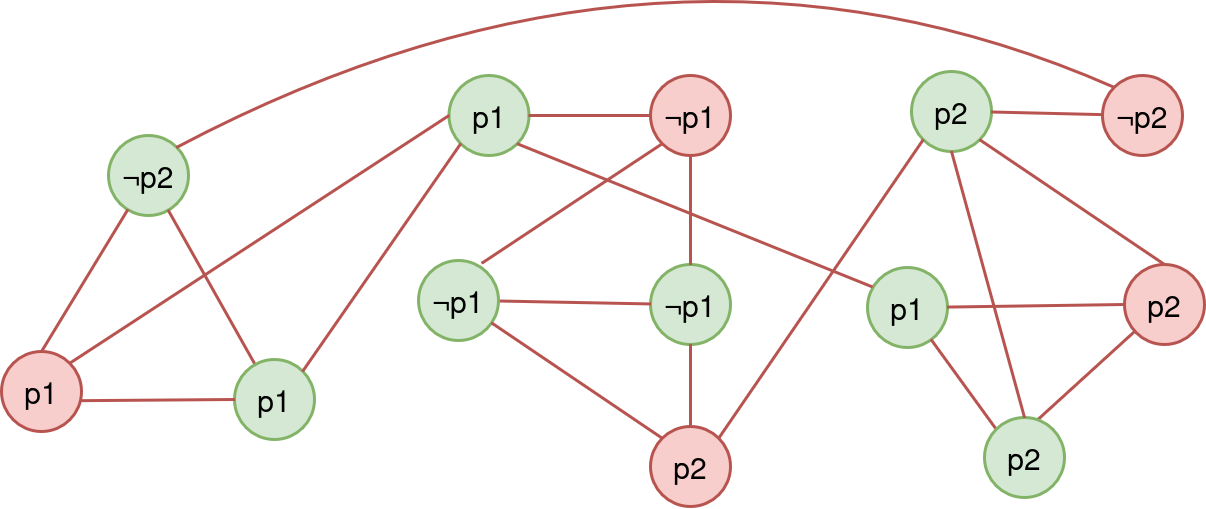
\includegraphics[width=0.55\linewidth]{images/T2_3_cobertura.png}
        \caption{Cobertura de k nodos del $G_\Phi$}
        \label{fig:enter-label}
    \end{figure}
\end{frame}




\end{document}
